\documentclass[12pt]{article}
\usepackage[utf8]{inputenc}
\usepackage{geometry}
\usepackage{lipsum}
% Bibliography in APS style (biblatex-phys). Build: pdflatex, biber, pdflatex, pdflatex.
\usepackage[style=phys,biblabel=brackets,articletitle=false,chaptertitle=false,pageranges=false,%
            sorting=none,doi=false,isbn=false,url=false,eprint=false]{biblatex}
\usepackage{amsmath}
\usepackage{amsfonts}
\usepackage{dsfont}
\usepackage{bbm}
\usepackage{graphicx}
\usepackage{bm}
\usepackage{physics}
\usepackage{titlesec}
%\usepackage{subfig}
\usepackage{listings}
\usepackage{xcolor}
\usepackage{tocloft}
\usepackage{pdfpages}
\usepackage{mathdots}
\addbibresource{Bibliography.bib}

\definecolor{codegreen}{rgb}{0.415,0.6,0.3294}
\definecolor{codegray}{rgb}{0.5,0.5,0.5}
\definecolor{codepurple}{rgb}{0.58,0,0.82}
\definecolor{codeblue}{rgb}{0.3333,0.5,0.824}
\definecolor{codered}{rgb}{0.6588,0.345,0.208}
\definecolor{backcolour}{rgb}{1.,1.,1.}

\lstdefinestyle{mystyle}{
    backgroundcolor=\color{backcolour},   
    commentstyle=\color{codegreen},
    keywordstyle=\color{codeblue},
    numberstyle=\tiny\color{codegray},
    stringstyle=\color{codered},
    basicstyle=\ttfamily\footnotesize,
    breakatwhitespace=false,         
    breaklines=true,                 
    captionpos=b,                    
    keepspaces=true,                 
    numbers=left,                    
    numbersep=5pt,                  
    showspaces=false,                
    showstringspaces=false,
    showtabs=false,                  
    tabsize=2
}

\lstset{style=mystyle}


\setcounter{secnumdepth}{4}

\titleformat{\paragraph}
{\normalfont\normalsize\bfseries}{\theparagraph}{1em}{}
\titlespacing*{\paragraph}
{0pt}{3.25ex plus 1ex minus .2ex}{1.5ex plus .2ex}

\begin{document}

\setlength{\cftpartindent}{0em}
\setlength{\cftsecindent}{0em}
\setlength{\cftsubsecindent}{0em}
\setlength{\cftsubsubsecindent}{0em}

\tableofcontents

\pagebreak

\section{Abel Transformation}
\begin{figure}[ht!]
    \centering
    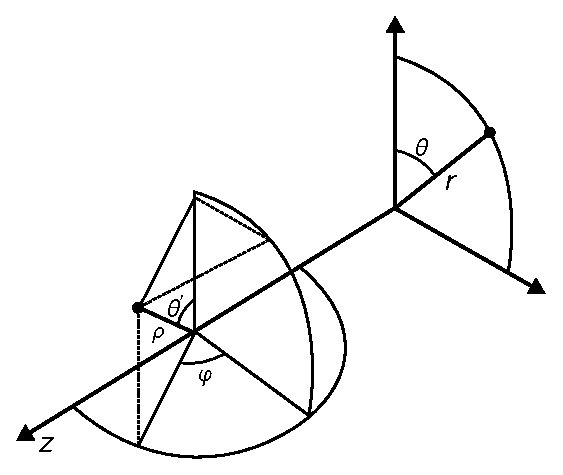
\includegraphics[width=0.6\linewidth]{Coordinates.eps}
    \caption{Illustration of spherical and polar coordinates}
    \label{fig:abel_coordinates}
\end{figure}
For a spherical distribution of intensity, a so-called Newton's sphere, in coordinates $\rho$, $\theta^\prime$, $\phi$, define the intensity $I(\rho,\theta^\prime,\phi)$. The Abel transformation is the projection of this distribution along an axis ($z$-axis) to a plane, given in polar coordinates $r$, $\theta$. One way of doing such a transformation is to make a BAsis Set EXpansion (BASEX) of $I(\rho,\theta^\prime,\phi)$ into some well defined basis set, from which the projection can be done. 
\subsection{rBASEX}
The rBASEX method described by Ryazanov \cite{ryazanov_development_2012} and implemented and discussed by Gibson et al. \cite{gibson_stephen_pyabelpyabel_2022} assumes a cylindrically symmetric distribution about an axis that lies in the plane of projection (the laser axis), from which $\theta^\prime$ and $\theta$ are measured. The projection axis $z$ cannot be the symmetry axis, since the projection along a symmetry axis would not depend on $\theta$. Thus, the intensity distribution is independent of the azimuthal angle $\phi$ around the symmetry axis and Ryazanov argues for a basis-set where $\rho$ and $\theta^\prime$ decouple,
\begin{equation*}
    b_{R;n}(\rho,\theta^\prime,\phi)=b_{R}(\rho)\cos^n(\theta^\prime),
\end{equation*}
with,
\begin{equation*}
    b_R(\rho)=\left\{
     \begin{array}{@{}l@{\thinspace}l}
       \rho-(R-1),\hspace{3mm}\text{for }R-1<\rho<R,\\
       R+1-\rho,\hspace{6.5mm}\text{for }R\leq\rho<R+1,\\
       0,\hspace{22mm}\text{otherwise.}\\
     \end{array}
   \right.
\end{equation*}
Then an expansion in the set $b_{R;n}(\rho,\theta^\prime,\phi)$ can be written as,
\begin{equation*}
    I(\rho,\theta^\prime,\phi)=\sum_{R,n}c_{R;n}b_{R;n}(\rho,\theta^\prime,\phi)=\sum_{n}I_n(\rho)\cos^n(\theta^\prime).
\end{equation*}
$I_n(\rho)=\sum_{R}c_{R;n}b_R(\rho)$ is then the radial distribution of intensity for each order of angular power in $\cos(\theta^\prime)$. The basis-set has a well defined projection onto the plane, where the radial and angular part also decouple to
\begin{equation*}
    p_{R;n}(r,\theta)=p_{R;n}(r)\cos^n(\theta).
\end{equation*}
Analogously, one can write the projected intensity distribution $P(r,\theta)$ as an expansion,
\begin{equation*}
    P(r,\theta)=\sum_{R,n}c_{R;n}p_{R;n}(r,\theta)=\sum_{n}P_n(r)\cos^n(\theta),
\end{equation*}
where $P_n(r)=\sum_{R}c_{R;n}p_{R;n}(r)$ is the projected radial intensity distribution for each angular order of $\cos(\theta)$. Notice that even though the basis set is not smooth the projections are \cite{ryazanov_development_2012,gibson_stephen_pyabelpyabel_2022}. Numerically one samples at integer radii $R$, which leaves $b_R(R)=1$ and zero otherwise, thus $I_n(\rho)=c_{\rho;n}$. Losing the subscript $\rho$ on the coefficients and writing it in matrix form,
\begin{align*}
    P_n(\bm{r})&=\bm{p}_n^TI_n(\bm{\rho}),\\
    I_n(\bm{\rho})&=\left(\bm{p}_n^T\right)^{-1}P_n(\bm{r}).
\end{align*}
The first line is the Abel transformation and the second line is the inverse Abel transformation. $\bm{p}_n$ is purely a product of the choice of basis and only depends on the choice of sampling $R$. In order to attain $I(\rho,\theta^\prime,\phi)$, which has cylindrical symmetry, one can expand it in Legendre polynomials $\mathcal{P}_n(\cos(\theta^\prime))$ and make a transformation from,
\begin{equation}
     \sum_nI_n(\rho)\cos^n(\theta^\prime)\rightarrow\frac{I(\rho)}{4\pi\rho^2}\sum_n\beta_n(\rho)\mathcal{P}_n(\cos(\theta^\prime)),\qquad\beta_0=1,
     \label{eq:intensity_harmonic_expanded}
\end{equation}
where $I(\rho)$ is the radial intensity distribution, whose integral $\int I(\rho)\,\mathrm{d}\rho$ is the total intensity, and $\beta_n(\rho)$ are the anisotropy parameters. All orders higher than $n=0$ describe the deviation from a completely spherically symmetric distribution. For further mathematical description confer Ryazanov \cite{ryazanov_development_2012} or Gibson et al. \cite{gibson_stephen_pyabelpyabel_2022}.
\section{Velocity Map Imaging}
Experimentally the distribution of interest is the velocity distribution of electrons ejected from an ion projected on a plane detector. Zare \cite{zare_photoejection_1972} has shown that for an ion in a thermal rotational initial distribution, ejection by $N$ photons yields angular intensity distributions with contributions by harmonics up to order $2N$. Cylindrical symmetry assumed by the rBASEX method is achieved by using a linearly polarized laser (or no laser) creating cylindrical symmetry along the laser polarization axis. Furthermore, reflection symmetry with respect to the perpendicular plane of the laser is expected \cite{ryazanov_development_2012}. Thus, the sum in eq. \ref{eq:intensity_harmonic_expanded} runs over the even orders from $0$ to $2N$.
\subsection{Image Distortions}
The detected projections usually differ from perfectly centered projections of harmonic functions. Radial distortions are very pronounced in measured data as-well as off-centering of the whole image. In order to combat these effects centering and circularization of the image is performed. For reflective symmetric data along an axis the center of mass can be used to estimate the center of the projection. Circularization (inspired by Gibson et al. \cite{gibson_stephen_pyabelpyabel_2022}) is achieved by binning the data in $r$ and $\theta$ coordinates and comparing angular slices of radial data, while moving one slice by some multiplication factor radially and another in bin counts; and doing least square optimisation on the difference in bin counts at all radial values of the slice that was not moved, using cubic spline with first derivative restrictions as boundary conditions to interpolate the values of the moved spline. Of the two parameters used in the optimisation only the radial correction factor is of interest, but omission of the bin count correction factor results in poor optimisation results. Further development could include error estimation of the correction factors.\\
Apart from distortions, detector efficiency is not perfectly equal at all values of the plane of projection. However, imposing the constraint that the projection must have reflective symmetry along the laser axis one can fold the image along the laser axis and achieve perfect reflective symmetry.
\subsection{Data analysis with rBASEX}
Recording the data of the projected intensity distribution can in literature be found done with cameras creating binned two dimensional data \cite{gibson_stephen_pyabelpyabel_2022,marion_autodetachment_2020}. However, with a MCP-RAE technique such as described by Saha et al. \cite{saha_experimental_2017} each projected emission from the intensity distribution can be recorded as point positions on the projection plane. Given a data-set of values $\bm{X}$ and $\bm{Y}$ in Cartesian coordinates, with a well defined center at $(x_c,y_c)$ and polar symmetry, denote the data-set's binning of angular order $n$ in radial space $d_n(\bm{r})$. Then for a given set of coordinates $(x_i,y_i)$, with radius $r_i$ defined as $\left((x_i-x_c)^2+(y_i-y_c)^2\right)^{1/2}$ times a correction factor from circularization, which falls in between $r$ and $r+\Delta r$ of vector $\bm{r}$ the contribution to $d_{nr}$ and $d_{n,r+\Delta r}$ is defined as,
\begin{align*}
    \cos^n(\theta_i)\left[1-\frac{|r-r_i|}{\Delta r}\right],\\
    \cos^n(\theta_i)\frac{|r-r_i|}{\Delta r},
\end{align*}
respectively; where,
\begin{align*}
    \cos(\theta_i)=\frac{y_i-y_c}{\left((x_i-x_c)^2+(y_i-y_c)^2\right)^{1/2}}.
\end{align*}
That is, the data is linearly radially binned with weights $\cos^n(\theta_i)$. Since $\cos(\theta_i)$ depends on $x_i-x_c$ only through $r_i$, it is unchanged by the reflection $x_i-x_c\rightarrow-(x_i-x_c)$ about the $y-y_c$ axis; aligning this axis with the axis of the laser therefore effectively folds the image as previously described. \\
The following implementation is inspired by Gibson et al. \cite{gibson_stephen_pyabelpyabel_2022}. Computationally it is advantageous to operate on coefficients of expansions. In order to get the coefficients of each angular order with respect to a uniform distribution, consider the conversion matrix $\bm{H}$, defined for each radius $r$ as the inverse of the Hankel matrix
\begin{equation*}
    \bm{d}_{r\text{ Hankel}}=\mqty(\sum_i\cos^0\theta_i & \sum_i\cos\theta_i & \cdots & \sum_i\cos^{n_{\max}}\theta_i \\
    \sum_i\cos\theta_i & \sum_i\cos^2\theta_i & \iddots & \vdots \\
    \vdots & \iddots & \iddots & \vdots \\
    \sum_i\cos^{n_{\max}}\theta_i & \sum_i\cos^{n_{\max}+1}\theta_i & \cdots & \sum_i\cos^{2n_{\max}}\theta_i),
\end{equation*}
with elements $\sum_i\cos^{n+m}\theta_i$ for $n,m=0,\ldots,n_{\max}$, where $n_{\max}$ is the highest angular order. For each $r$ the sum runs over angles $\theta_i$ separating equally sized areas in the radial slice of $r$, as shown in figure \ref{fig:HankelBins}.
\begin{figure}[ht!]
    \centering
    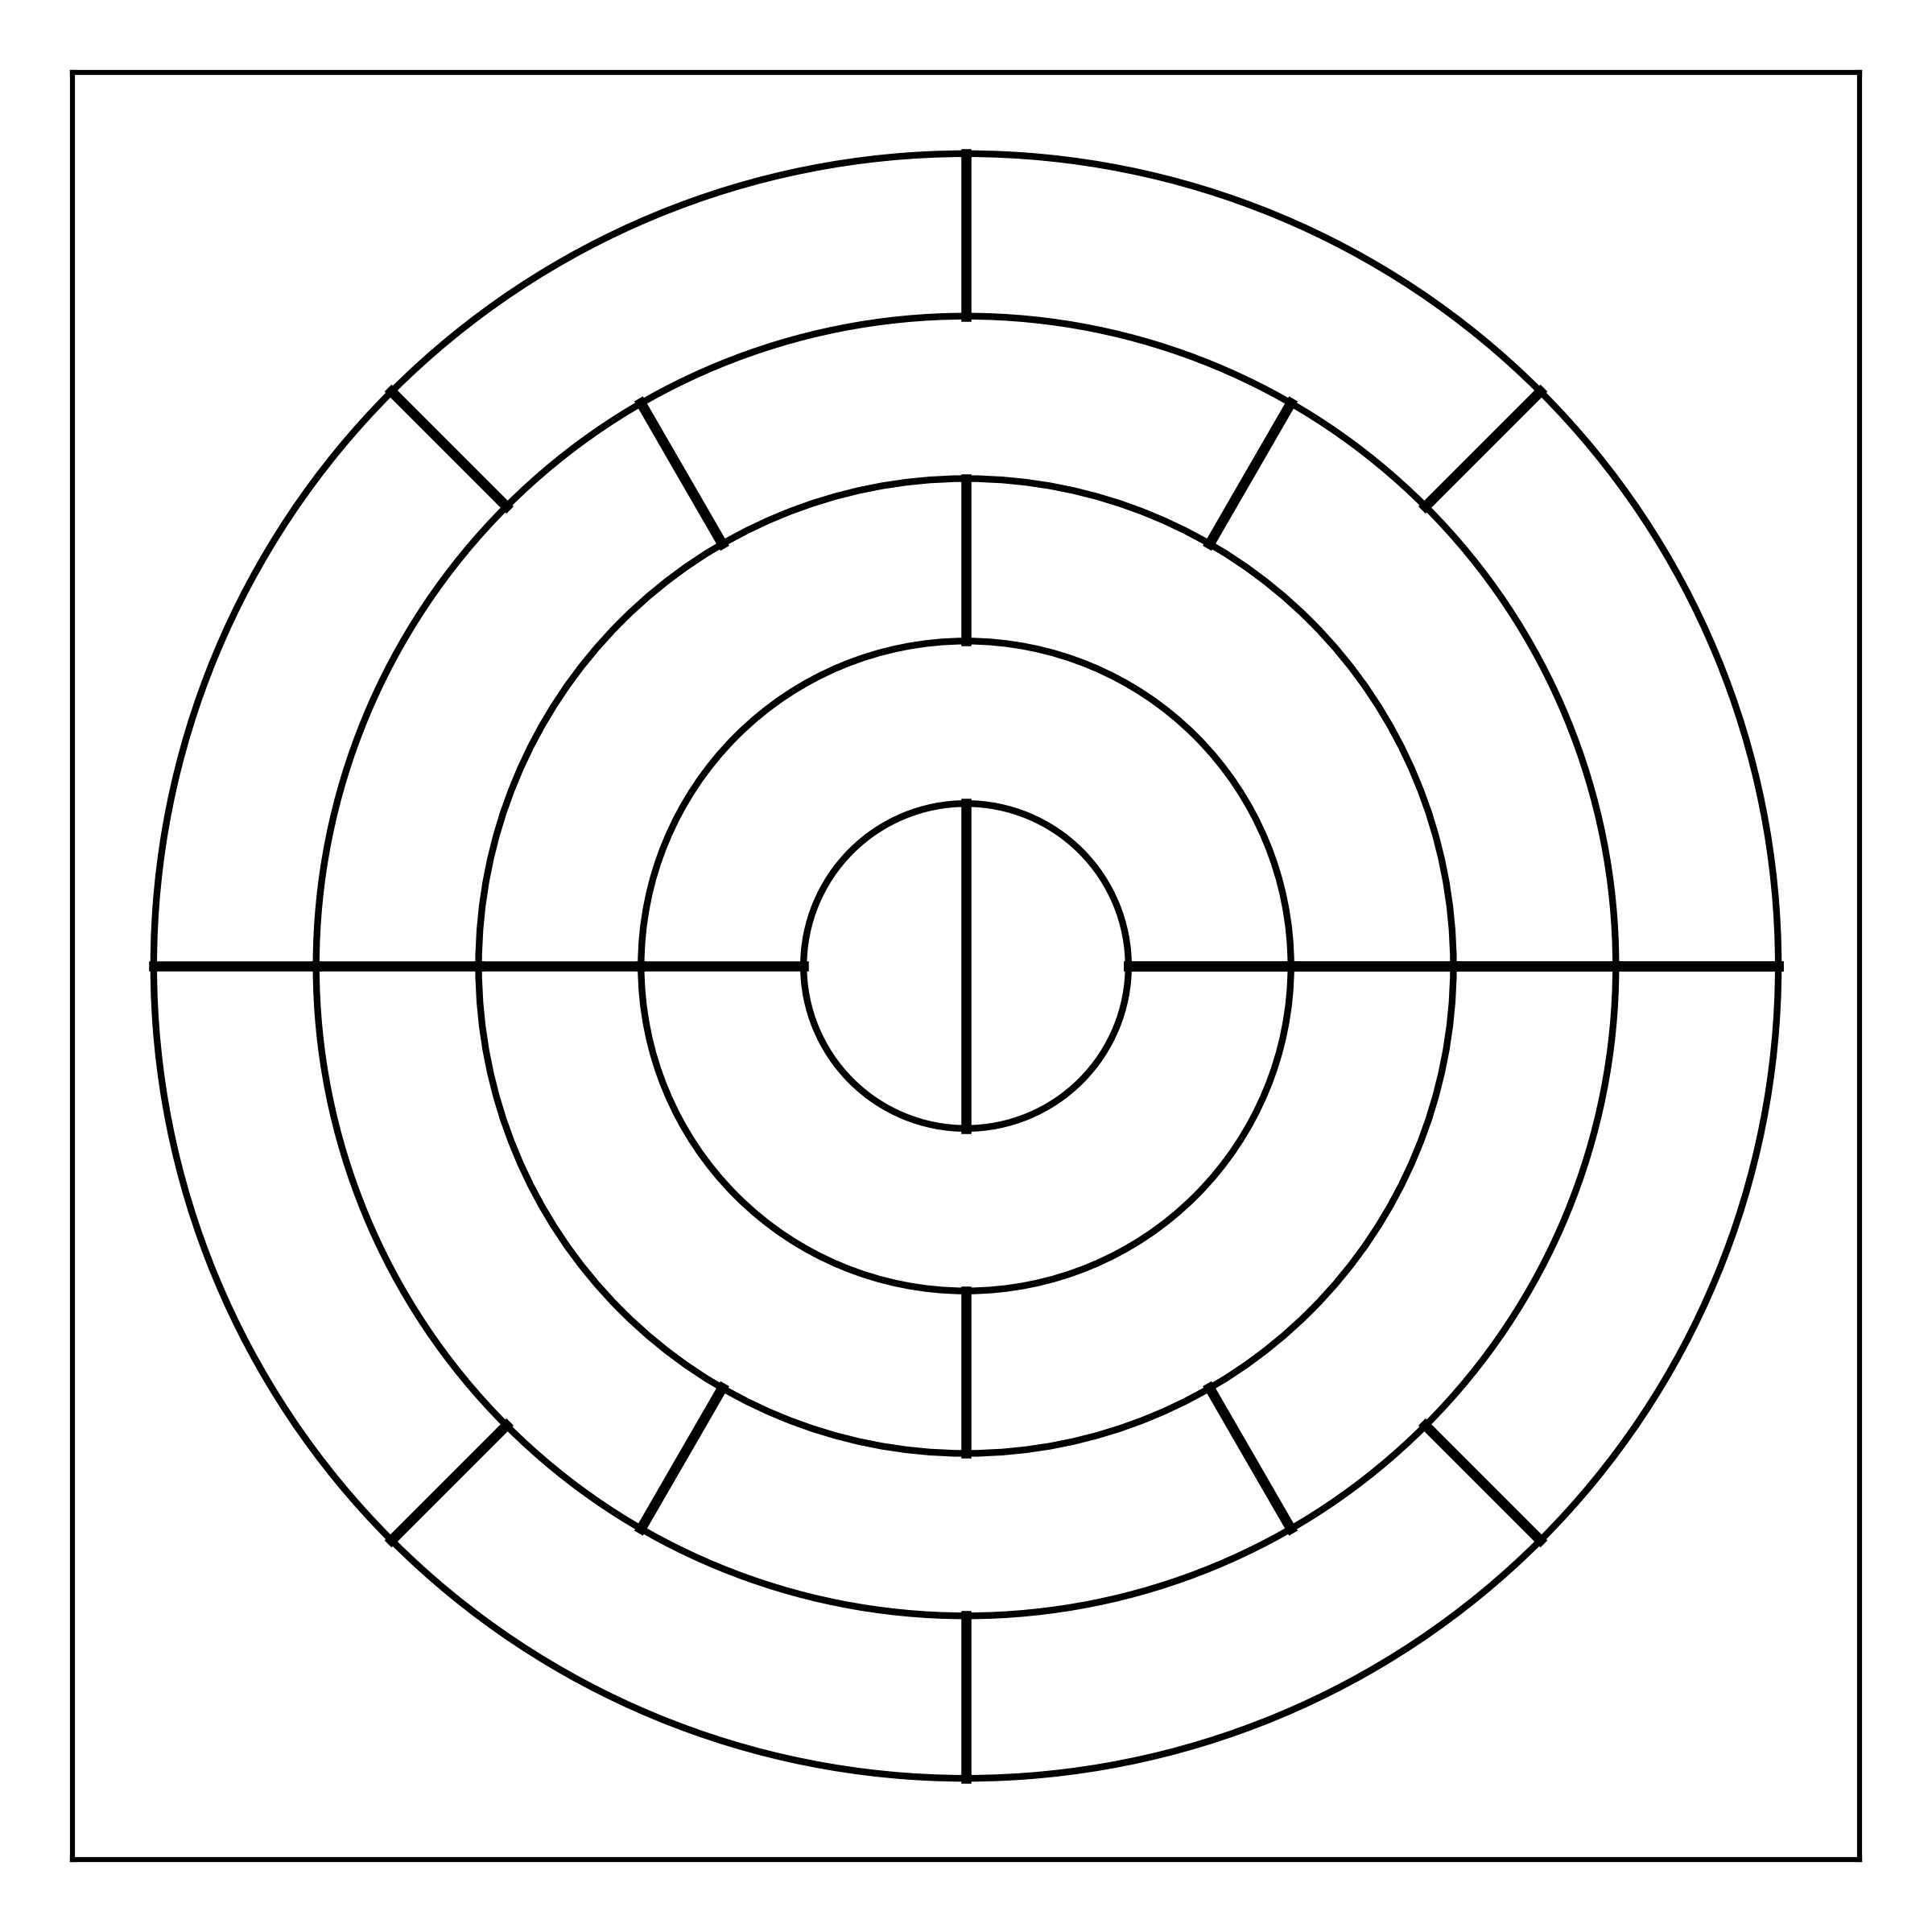
\includegraphics[width=0.4\linewidth]{HankelBins.png}
    \caption{Radial lines represent angles $\theta_i$ to use in the sum $\sum_i\cos^n\theta_i$ for each radial bin, represented by the drawn circles.}
    \label{fig:HankelBins}
\end{figure}
The area $A$ attributed to one angle can be chosen arbitrarily; a natural choice is $A=\pi\Delta r^2$. It only sets the overall scale of the coefficients. The number of angles in a slice is the area of the slice divided by $A$. The events are shared between neighbouring bins with the weights above, so the slice of $r=j\Delta r$ has the area $2\pi j\Delta r^2$ for $j\geq1$ (and $2\pi\Delta r^2/6$ for the one-sided slice at $r=0$, where $j$ is replaced by $1/6$). In the limit of many angles the sums are therefore
\begin{equation*}
    \sum_i\cos^{n+m}\theta_i\;\rightarrow\;\frac{j\,\Delta r^2}{A}\oint_0^{2\pi}\cos^{n+m}\theta\,\mathrm{d}\theta,
\end{equation*}
which depends on $n+m$ only, as a Hankel matrix does, and $\bm{H}$ is its exact inverse. No integer number of angles is needed, and no element of $\bm{H}$ is treated differently from the others. Using this, the projected radial intensity distribution $P_n(\bm{r})$ is written as,
\begin{equation*}
    P_{nr}=\sum_{i}H_{rni}d_{ir}
\end{equation*}
and the inverse Abel transformation can be calculated using the basis-set of rBASEX to find $\left(\bm{p}_n^T\right)^{-1}$ as,
\begin{equation*}
    I_{n\rho}=\sum_{j}\left(p^T\right)_{\rho j;n}^{-1}\sum_{i}H_{jni}d_{ij}.
\end{equation*}
As described above, instead of summing $I_n(\bm{\rho})$ over $\cos^n(\theta^\prime)$ expanding it in Legendre polynomials instead yields both the total radial intensity distribution $I(\bm{\rho})$ and the anisotropy of the distribution. Thus, consider the matrix $\bm{C}$ consisting of the coefficients of the first $n$ Legendre polynomials in its columns. Then,
\begin{equation*}
    \sum_{i}C^{-1}_{ni}I_{i\rho}=\sum_{k}C^{-1}_{nk}\sum_{j}\left(p^T\right)_{\rho j;k}^{-1}\sum_{i}H_{jki}d_{ij},
\end{equation*}
leaves the coefficients for an expansion in $n$ Legendre polynomials at coordinate $\rho$, where the 0'th term is $I(\rho)/(4\pi\rho^2)$. Integrating over $\theta^\prime$ and $\phi$ with the volume element $\rho^2\,\mathrm{d}\rho\,\mathrm{d}\Omega$ leaves,
\begin{equation*}
    I(\rho)=4\pi\rho^2\sum_{k}C^{-1}_{0k}\sum_{j}\left(p^T\right)_{\rho j;k}^{-1}\sum_{i}H_{jki}d_{ij}.
\end{equation*}
All matrices are purely dependent on the amount of bins and angular orders considered.
\subsubsection{Error estimation}
Error estimation is paramount in order to analyse the intensity distribution calculated by Abel inversion. For error propagation, denote the variance correlation matrix for binned data $\bm{\Sigma^c}_n$
\begin{equation*}
    \bm{\Sigma^c}_n=\mqty(\sigma_{d_{n1}}^2 & \sigma_{d_{n1}d_{n2}} & \sigma_{d_{n1}d_{n3}} & \cdots\\
                     \sigma_{d_{n2}d_{n1}} & \sigma_{d_{n2}}^2 & \sigma_{d_{n2}d_{n3}} & \cdots\\
                     \sigma_{d_{n3}d_{n1}} & \sigma_{d_{n3}d_{n2}} & \sigma_{d_{n3}}^2 & \cdots\\
                     \vdots & \vdots & \vdots & \ddots),
\end{equation*}
and the Jacobian of the set of points $I(\bm{\rho})$
\begin{equation*}
    \bm{J}_n=\mqty(\frac{\partial I_{1}}{\partial d_{n1}} & \frac{\partial I_{1}}{\partial d_{n2}} & \frac{\partial I_{1}}{\partial d_{n3}} & \cdots \\
    \frac{\partial I_{2}}{\partial d_{n1}} & \frac{\partial I_{2}}{\partial d_{n2}} & \frac{\partial I_{2}}{\partial d_{n3}} & \cdots \\
    \frac{\partial I_{3}}{\partial d_{n1}} & \frac{\partial I_{3}}{\partial d_{n2}} & \frac{\partial I_{3}}{\partial d_{n3}} & \cdots \\
    \vdots & \vdots & \vdots & \ddots ),
\end{equation*}
where
\begin{equation*}
    \frac{\partial I(\rho_{i})}{\partial d_{nj}} = 4\pi\rho_i^2\sum_{z}C^{-1}_{0z}\left(p^T\right)_{ij;z}^{-1}H_{jzn}.
\end{equation*}
Then the variance correlation matrix $\bm{\Sigma^I}_n$ of a set $\bm{I}_n$ is given by,
\begin{equation*}
    \bm{\Sigma^I}_n=\bm{J}_n\bm{\Sigma^c}_n\bm{J}_n^T=\mqty(\sigma_{I_{1,n}}^2 & \sigma_{I_{12,n}} & \sigma_{I_{13,n}} & \cdots\\
                     \sigma_{I_{21,n}} & \sigma_{I_{2,n}}^2 & \sigma_{I_{23,n}} & \cdots\\
                     \sigma_{I_{31,n}} & \sigma_{I_{32,n}} & \sigma_{I_{3,n}}^2 & \cdots\\
                     \vdots & \vdots & \vdots & \ddots).
\end{equation*}
Assuming no correlation between bins variance in $I(\rho_i)$ is,
\begin{equation*}
    \sigma_{I_{i}}^2=\sum_{n}\Sigma_{ii,n}^I=\sum_{k,l,n}J_{ik,n}\Sigma^c_{kl,n}J_{il,n}\rightarrow \sum_{k,n}J_{ik,n}\sigma_{d_{nk}}^2J_{ik,n}.
\end{equation*}
Contributions to $\sigma^2_{d_{nk}}$ considered are from errors in $\bm{X}$, $\bm{Y}$ and the center $(x_c,y_c)$. Without correlation effects,
\begin{align*}
    \sigma^2_{d_{nk}}=\sum_{i} & \left|\frac{\partial d_{nk}}{\partial x_i}\right|^2(\sigma_x^2+\sigma_{x_c}^2)+\left|\frac{\partial d_{nk}}{\partial y_i}\right|^2(\sigma_y^2+\sigma_{y_c}^2),
\end{align*}
for all $i$ points in bin $k$. This uses the fact that the binning method is linearly differentiable. \\
For systematic error in $X$ and $Y$ error propagation works, but there is no statistical error in $X$ and $Y$ and naively using the bin count $d_{nk}$ as $\sigma^2_{d_{nk}}$ fails to produce realistic errors. For large data sets an estimate of the error in the intensity distribution can be found by bootstrapping the data set \cite{efron_bootstrap_1985,efron_nonparametric_1981}. Results of bootstrapping are highly dependent on the chosen angular order and number of bins. However, for large number of re-samples each statistic from the intensity distribution vector's $\hat{\bm{I}}$ distribution of bootstrap statistics $\hat{\bm{I}}_B$ are normal distributed with bias. Therefore, B. Efron's bias corrected bootstrap with a large number of re-samples is used to estimate $\pm1\sigma$ confidence intervals, with the confidence level $1-2\Phi(-1)\approx68.3\,\%$, where $\Phi$ is the cumulative distribution function of a standard normal distribution \cite{efron_better_1987,efron_transformation_1982,efron_bootstrap_1985}. The confidence intervals are used as asymmetric errors with respect to the measured statistic $\hat{\bm{I}}$. From tests on experimental data, the number of re-samples usually needed to produce well defined normal distributions of $\hat{\bm{I}}_B$ are well above 5000. Further developments should test this method against simulated data.
\subsection{Calibration}
The inverse Abel transformation yields an intensity as a function of the 3D radius $\rho$ of a Newton sphere, which with rBASEX is equivalent to the 2D projection radius $r$. Blondel et al. \cite{blondel_photodetachment_1998} have shown that $r\propto\sqrt{E}$ where the energy $E$ is that of the electron. Thus, for a specific set of potentials projecting the detached electronic wavefunction onto the imaging plane (at a fixed distance), a calibration of the proportionality can be made with known energies and radii. A Gaussian distribution is expected from a measured intensity $I(\rho)$ of an electronic wavefunction with a specific energy. However, experimental data differs from a Gaussian distribution, with heavier tails of its distribution indicating that it is t-distributed. It is unclear where this broadening effect comes from, but the standard deviation and the center does not change if one assumes a t-distribution. Fitting to the data has been performed through minimization of,
\begin{equation*}
    \chi^2=\left(\bm{y}-f(\bm{x},\bm{p})\right)^T\left[\Sigma^c_y+J_x(\bm{x},\bm{p})\,\Sigma^c_x\,J_x(\bm{x},\bm{p})^T\right]^{-1}\left(\bm{y}-f(\bm{x},\bm{p})\right).
\end{equation*}
Where $\bm{x}$, $\bm{y}$ are the data, $f$ the function wished to fit and $\bm{p}$ its parameters, $J_x$ the Jacobian of $f$ with respect to $x$, and $\Sigma^c_{y,x}$ are the covariance matrices defined by the statistical error $\sigma$ and systematic error $s$ as,
\begin{equation*}
    \Sigma^c_{y,x}=\mqty(\sigma^2_1 + s^2_1 & s_1s_2 & \cdots & s_1s_N\\
    s_2s_1 & \sigma^2_2 + s^2_2 & \ddots & \vdots\\
    \vdots & \ddots & \ddots & \vdots\\
    s_Ns_1 & \cdots & \cdots & \sigma^2_N + s^2_N).
\end{equation*}
If all the systematic errors are equal, they are usually error propagated after fitting; however, the systematic error in the intensity due to systematic error in the coordinates are not equal between different radii \cite{hughes_measurements_2010}. Asymmetric errors in $y$ are accounted for by using the lower error (covariance matrix) when the sign of $y-f(x,\bm{p})$ is positive and vice versa. Thus, the normalized residuals are defined as,
\begin{equation*}
    \text{Norm. Res.}=\operatorname{sgn}\left(y_i-f(x_i,\bm{p})\right)\sqrt{\left|\left(y_i-f(x_i,\bm{p})\right)\left[\left[\Sigma^c_y+J_x\Sigma^c_xJ_x^T\right]^{-1}\left(\bm{y}-f(\bm{x},\bm{p})\right)\right]_i\right|},
\end{equation*}
with the sign determined by the sign of $\left(y_i-f(x_i,\bm{p})\right)$; the absolute value is needed because the product can be negative for a non diagonal covariance matrix. This definition of normalized residuals means that for non diagonal $\Sigma^c_{y,x}$ one cannot expect them to lie within $\pm1$ two thirds of the time, but Gaussian spread is still expected. Since both the systematic and statistical error in the radius is linear and respectively equal between all intensities, it is not used for fitting a t-distribution to $I(\rho)$ \cite{hughes_measurements_2010}.\\
\begin{figure}[t!]
    \centering
    {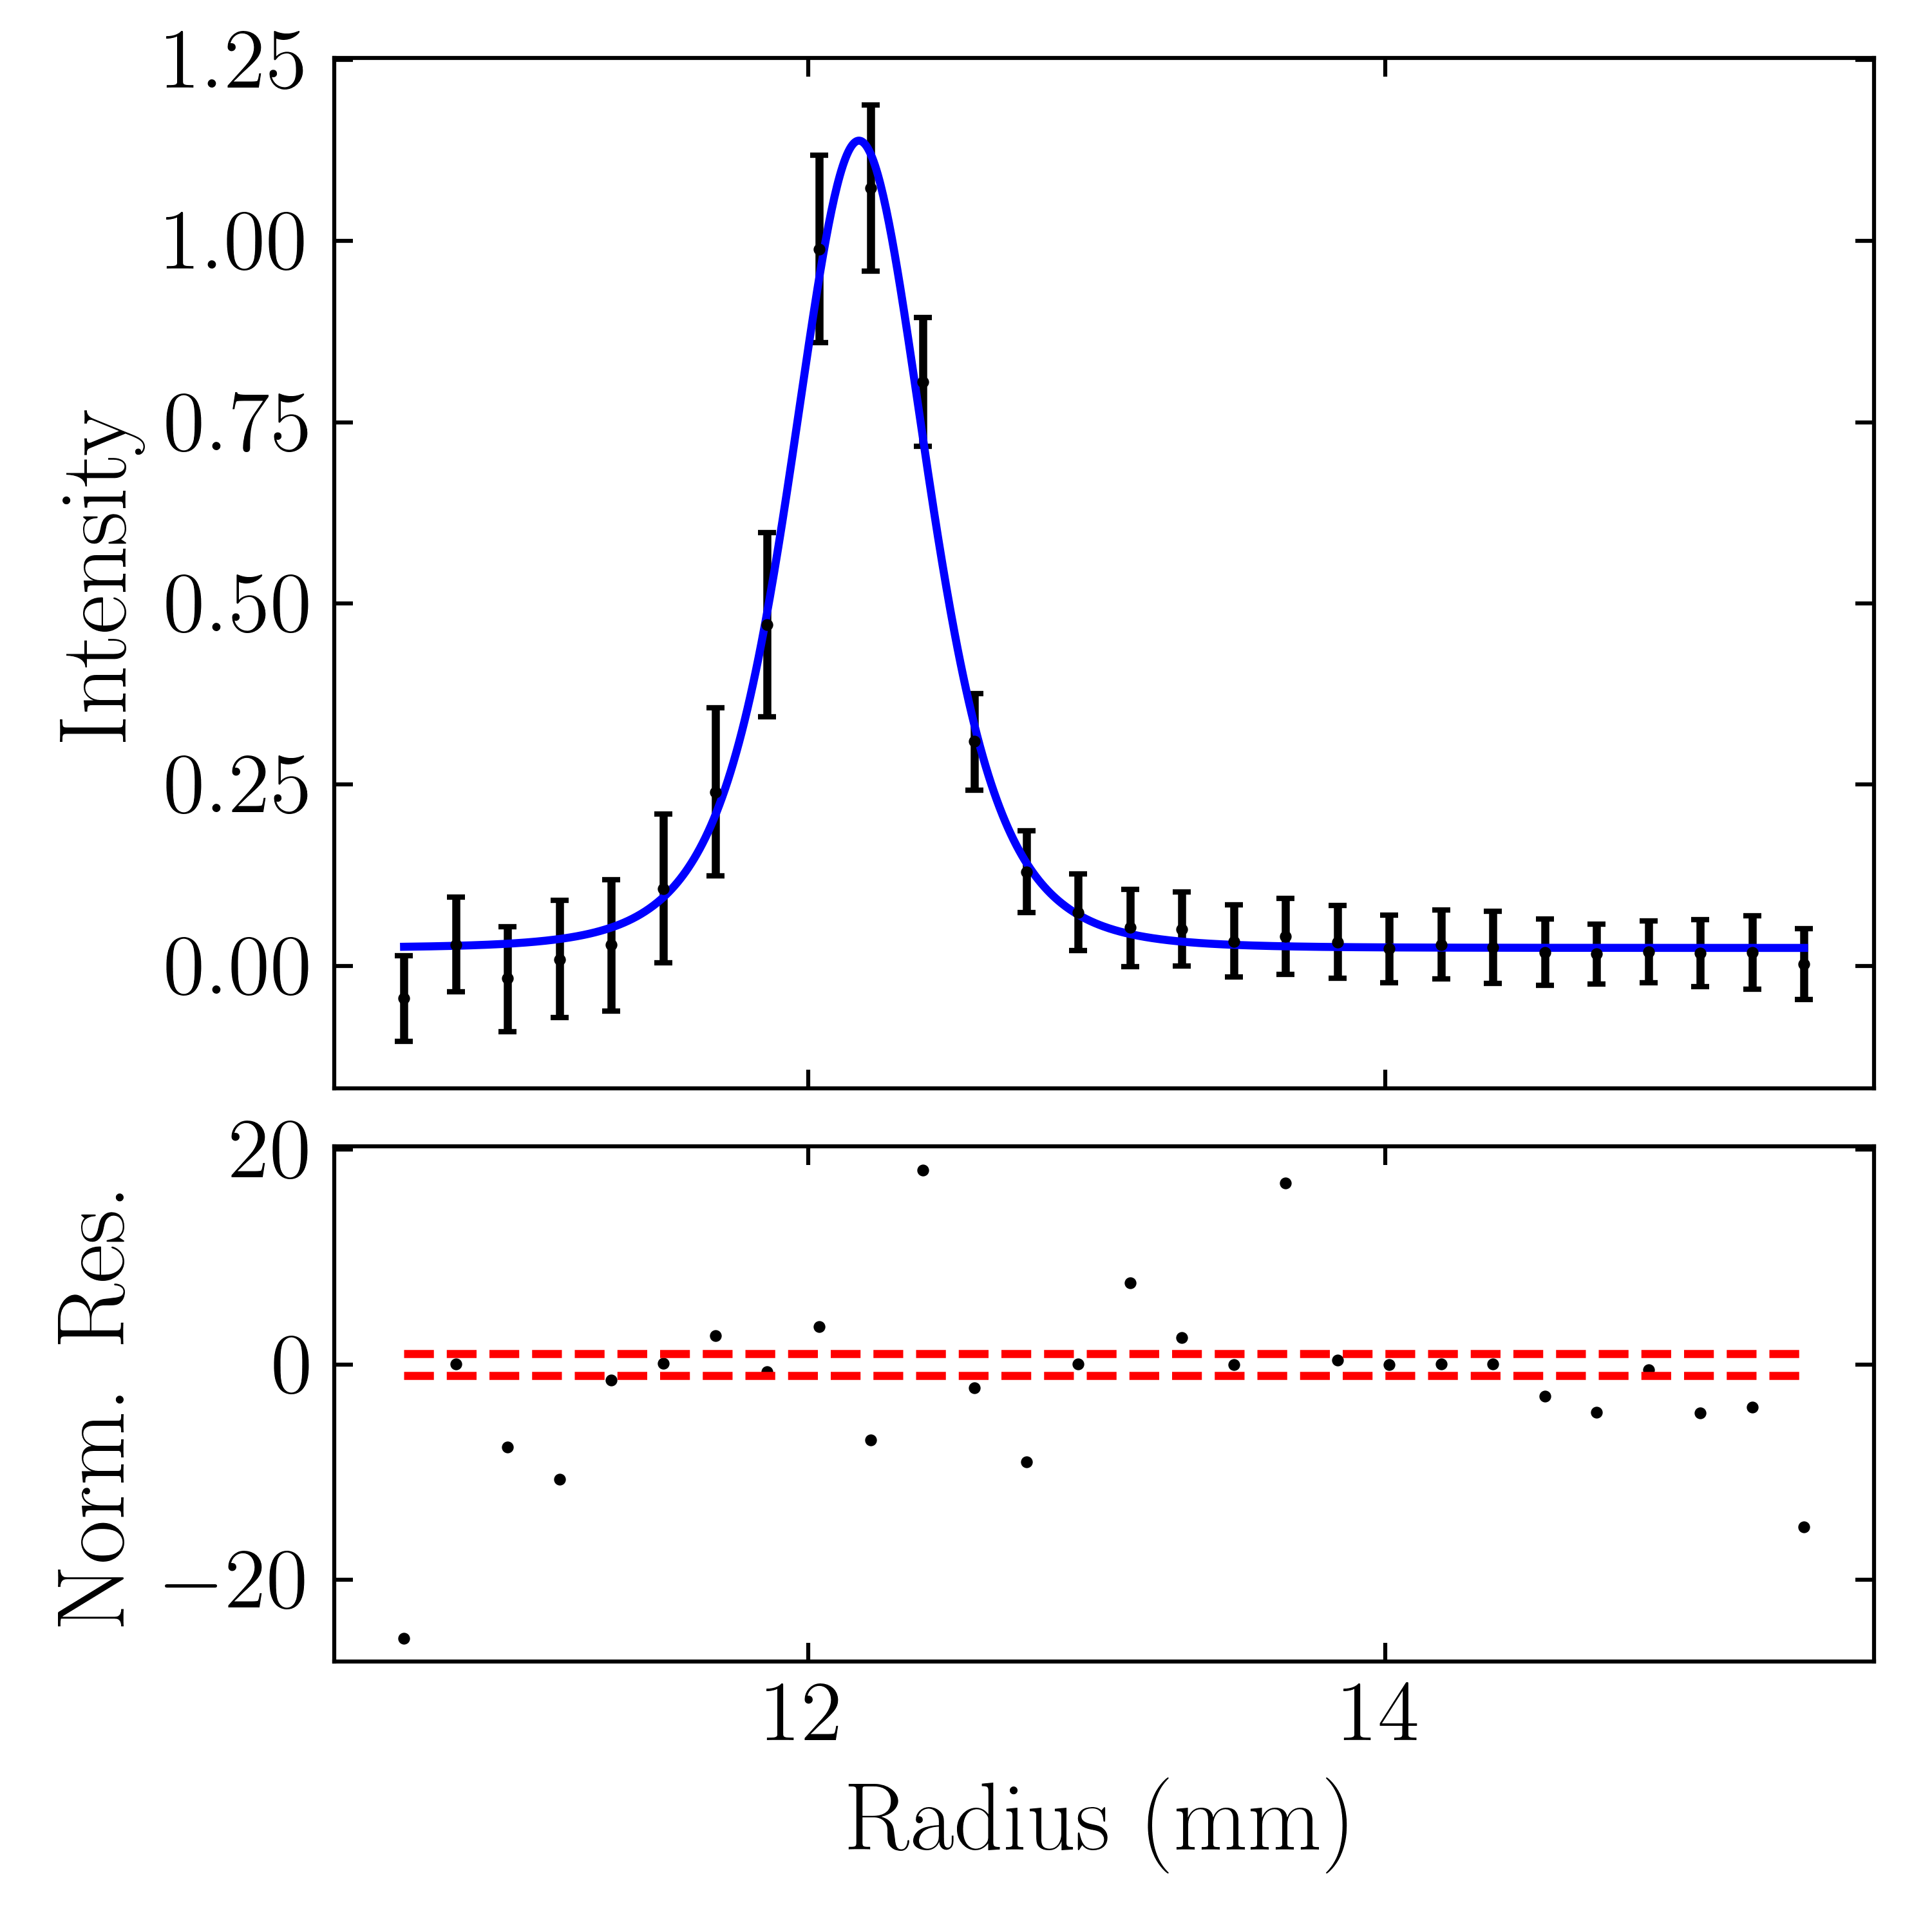
\includegraphics[width=0.49\linewidth]{thirdpeakCsfit.png}}
    {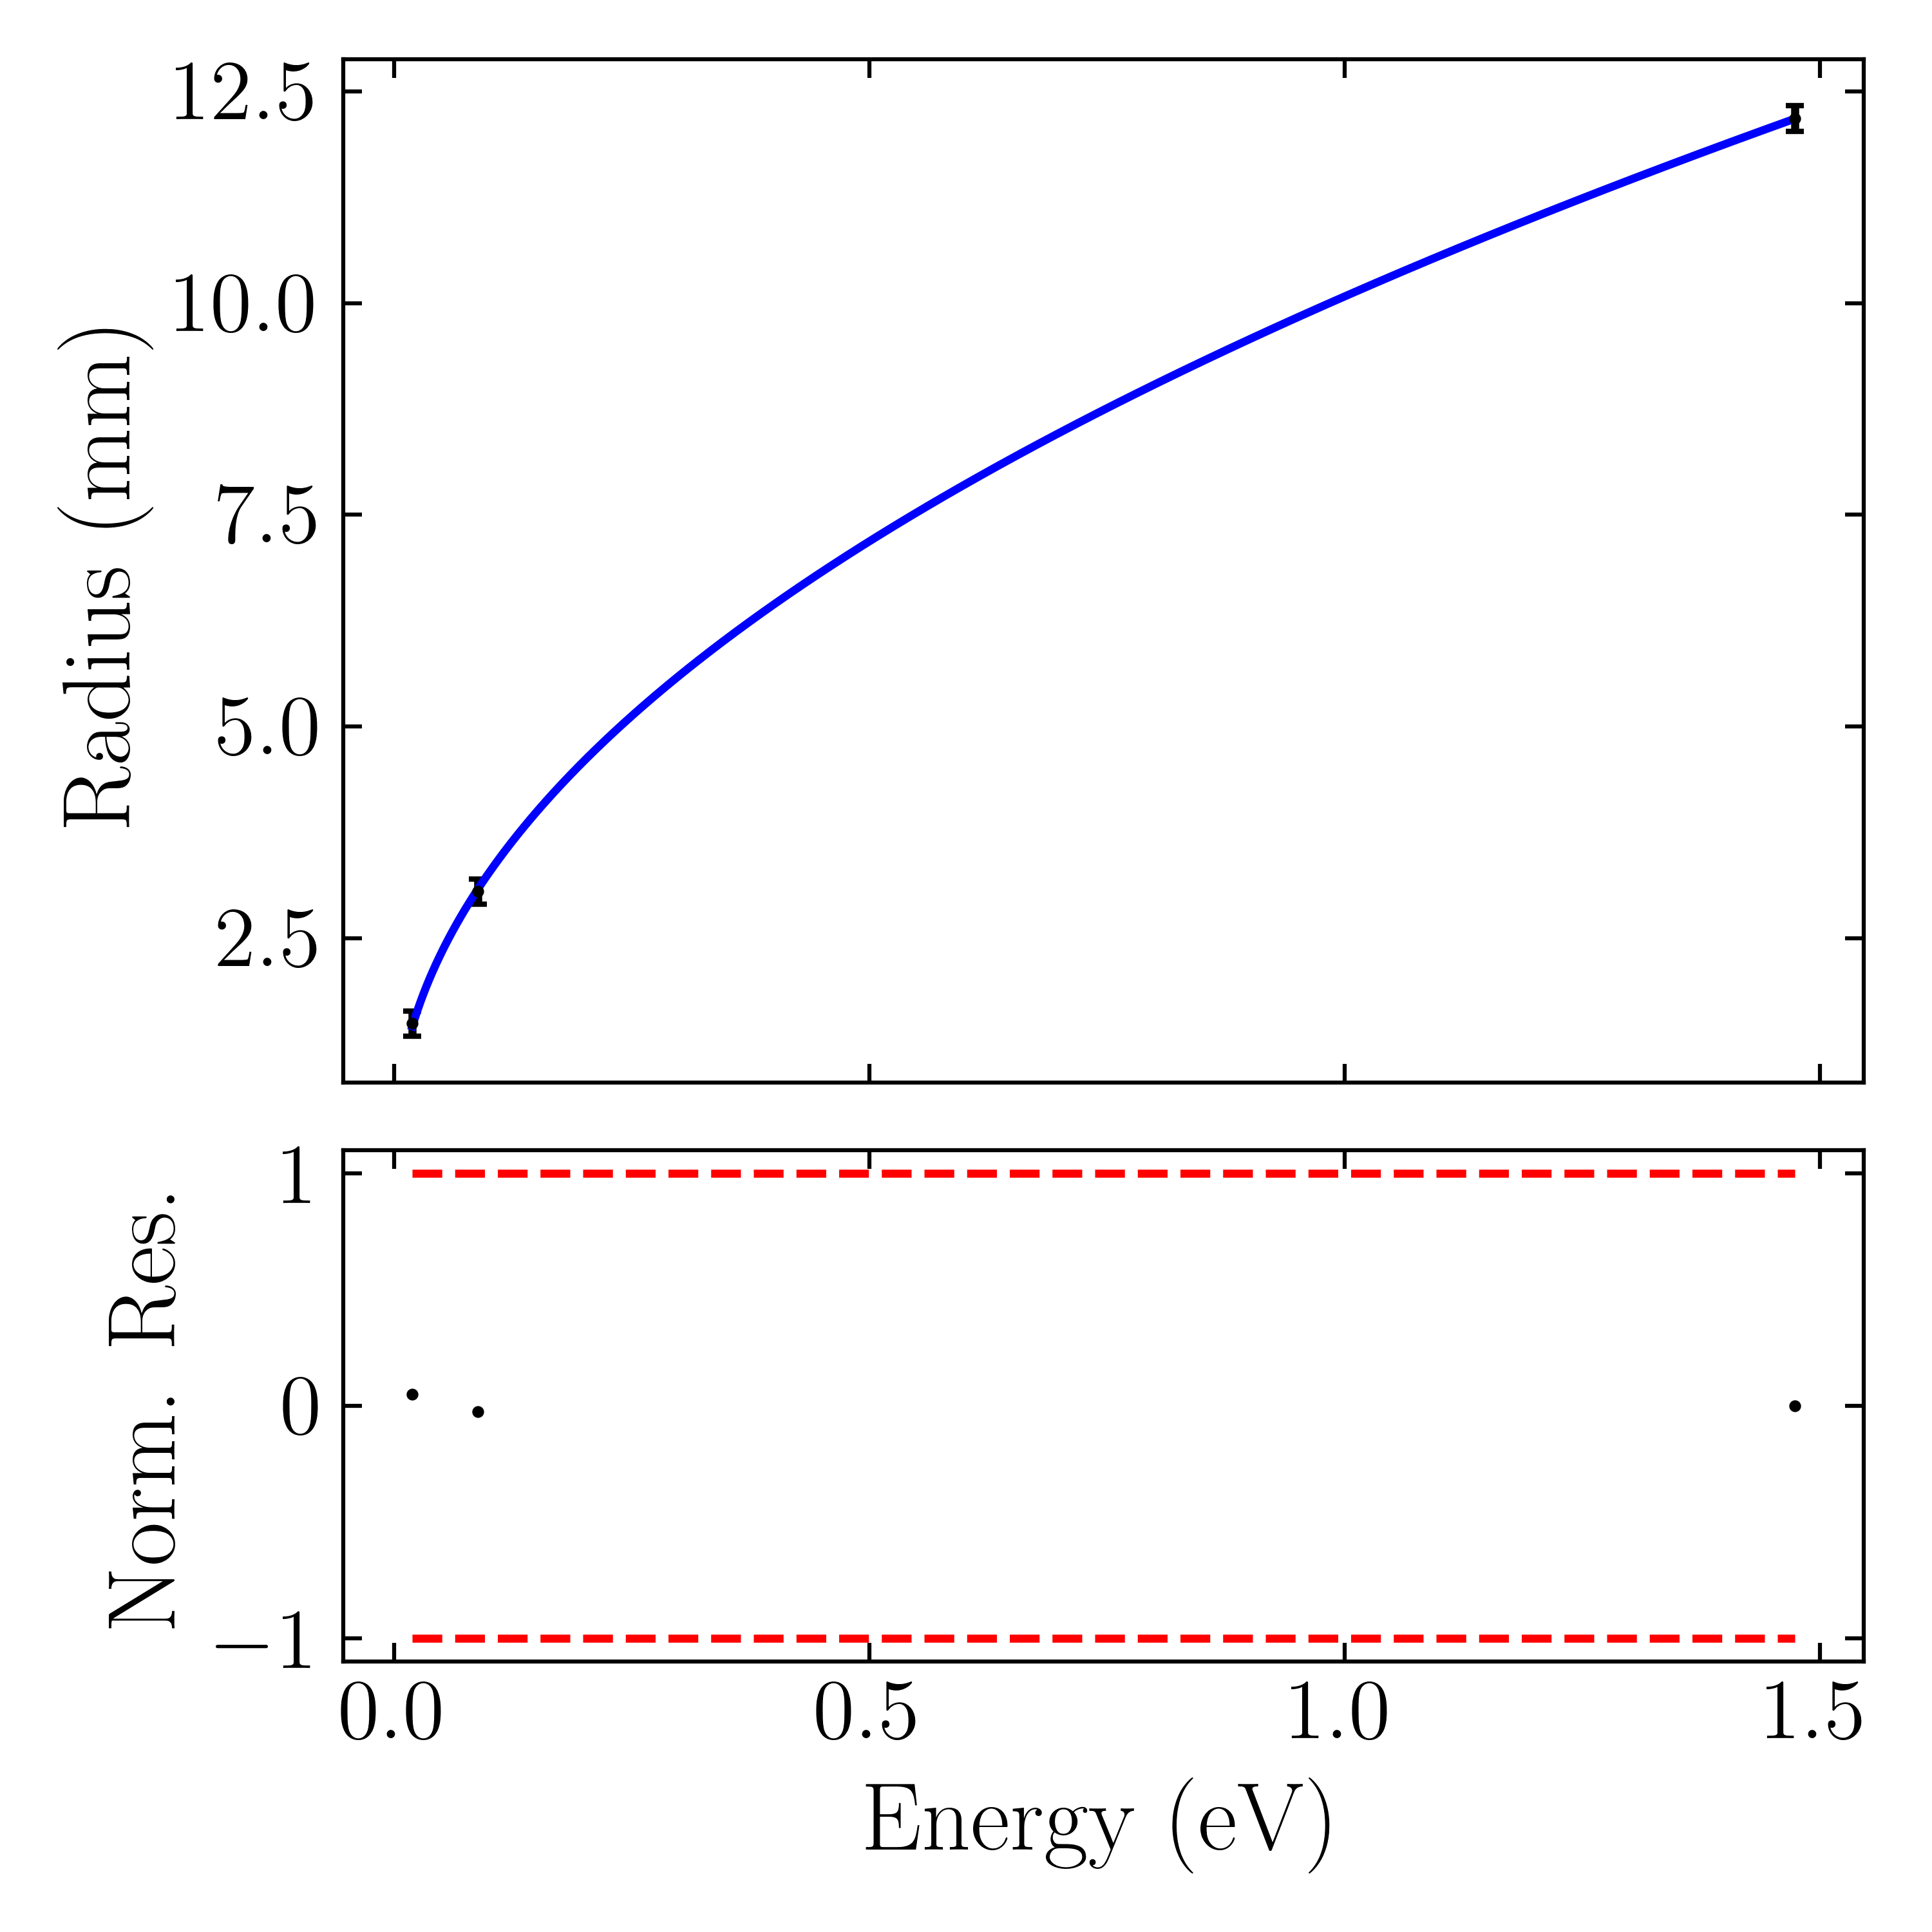
\includegraphics[width=0.49\linewidth]{CalibrationFit.png}}
    \caption{Left: Fit to a t-distribution, with minimization function and errors defined in the text. Plotted error bars are the square root of the diagonal of $\Sigma^c_y$. P-value$=0.10$. Right: Fit to $(E/a)^{1/b}$, where $E$ is the energy and $a$ and $b$ are fitting parameters. P-value$=0.79$.}
    \label{fig:calibration-fig}
\end{figure}
An example of a t-distribution fit from a ${}^{133}$Cs${}^{-}$ measurement can be seen on the left in figure \ref{fig:calibration-fig}. A 1.94542(3)eV laser was used to induce photoionization producing electron detachment to both ground state ${}^{133}$Cs and its $P_{1/2}$,$P_{3/2}$ states \cite{udem_absolute_1999,udem_absolute_2000,welander_field_2022}. It has been assumed that the systematic error in $\bm{X},\bm{Y}$ are $2\%$ of the 46 mm diameter MCP used in the MCP-RAE, while the statistical error has been calculated using bias corrected $\pm1\sigma$ ($68.3\,\%$) confidence interval of 5000 bootstrap samples. Due to fitting parameter sensitivity, the fit has been done with a differential evolution algorithm and the errors in the fitting parameters have been calculated using an analytical expression of the Hessian matrix of the t-distribution and numerically evaluated second derivative $\chi^2$. With a P-value of $0.10$ the fit is accepted to produce realistic errors with the mean of the distribution reported as $12.180(4)$ mm. However, one should add to this the statistical and systematic error in the radius which for calibration fitting is crucial, with the exception that the systematic error is equal among all measurements and can be neglected in fitting and error propagated afterwards. Thus, with the mean of each peak determined fitting to an inverse power law $(E/a)^{1/b}$ has been performed on the right in figure \ref{fig:calibration-fig}. Errors are again estimated using the Hessian of the function and with a P-value of $0.79$ are considered realistic. A power of $b=2.05(4)$ is consistent with Blondel et al.'s $r\propto\sqrt{E}$ and one could argue for fitting directly to $\sqrt{E/a}$.

\pagebreak

\printbibliography

\end{document}